\documentclass[14pt]{extbook}
\usepackage{multicol, enumerate, enumitem, hyperref, color, soul, setspace, parskip, fancyhdr} %General Packages
\usepackage{amssymb, amsthm, amsmath, bbm, latexsym, units, mathtools} %Math Packages
\everymath{\displaystyle} %All math in Display Style
% Packages with additional options
\usepackage[headsep=0.5cm,headheight=12pt, left=1 in,right= 1 in,top= 1 in,bottom= 1 in]{geometry}
\usepackage[usenames,dvipsnames]{xcolor}
\usepackage{dashrule}  % Package to use the command below to create lines between items
\newcommand{\litem}[1]{\item#1\hspace*{-1cm}\rule{\textwidth}{0.4pt}}
\pagestyle{fancy}
\lhead{Progress Quiz 8}
\chead{}
\rhead{Version B}
\lfoot{4553-3922}
\cfoot{}
\rfoot{Fall 2020}
\begin{document}

\begin{enumerate}
\litem{
Solve the quadratic equation below. Then, choose the intervals that the solutions $x_1$ and $x_2$ belong to, with $x_1 \leq x_2$.\[ 10x^{2} +57 x + 54 = 0 \]\begin{enumerate}[label=\Alph*.]
\item \( x_1 \in [-9.61, -8.33] \text{ and } x_2 \in [-0.67, -0.42] \)
\item \( x_1 \in [-45.06, -43.86] \text{ and } x_2 \in [-12.03, -11.96] \)
\item \( x_1 \in [-3.79, -2.7] \text{ and } x_2 \in [-1.51, -1.28] \)
\item \( x_1 \in [-6, -3.8] \text{ and } x_2 \in [-1.31, -1.17] \)
\item \( x_1 \in [-15.12, -12.2] \text{ and } x_2 \in [-0.5, -0.35] \)

\end{enumerate} }
\litem{
Solve the quadratic equation below. Then, choose the intervals that the solutions $x_1$ and $x_2$ belong to, with $x_1 \leq x_2$.\[ 12x^{2} +11 x -36 = 0 \]\begin{enumerate}[label=\Alph*.]
\item \( x_1 \in [-0.9, 0.02] \text{ and } x_2 \in [3.15, 4.67] \)
\item \( x_1 \in [-2.53, -1.56] \text{ and } x_2 \in [1.03, 1.47] \)
\item \( x_1 \in [-27.88, -25.28] \text{ and } x_2 \in [15.47, 16.58] \)
\item \( x_1 \in [-9.33, -7.37] \text{ and } x_2 \in [-0.25, 0.42] \)
\item \( x_1 \in [-4.87, -2.48] \text{ and } x_2 \in [0.65, 0.69] \)

\end{enumerate} }
\litem{
Factor the quadratic below. Then, choose the intervals that contain the constants in the form $(ax+b)(cx+d); b \leq d.$\[ 24x^{2} +38 x + 15 \]\begin{enumerate}[label=\Alph*.]
\item \( a \in [7.19, 9.72], \hspace*{5mm} b \in [3, 7], \hspace*{5mm} c \in [2.2, 4.2], \text{ and } \hspace*{5mm} d \in [0, 7] \)
\item \( a \in [3.28, 5.6], \hspace*{5mm} b \in [3, 7], \hspace*{5mm} c \in [5.3, 8.4], \text{ and } \hspace*{5mm} d \in [0, 7] \)
\item \( a \in [1.39, 3.83], \hspace*{5mm} b \in [3, 7], \hspace*{5mm} c \in [11.7, 13], \text{ and } \hspace*{5mm} d \in [0, 7] \)
\item \( a \in [0.35, 1.34], \hspace*{5mm} b \in [16, 24], \hspace*{5mm} c \in [-2.7, 1.5], \text{ and } \hspace*{5mm} d \in [16, 22] \)
\item \( \text{None of the above.} \)

\end{enumerate} }
\litem{
Graph the equation below.\[ f(x) = (x+4)^2 - 13 \]\begin{enumerate}[label=\Alph*.]
\begin{multicols}{2}\item 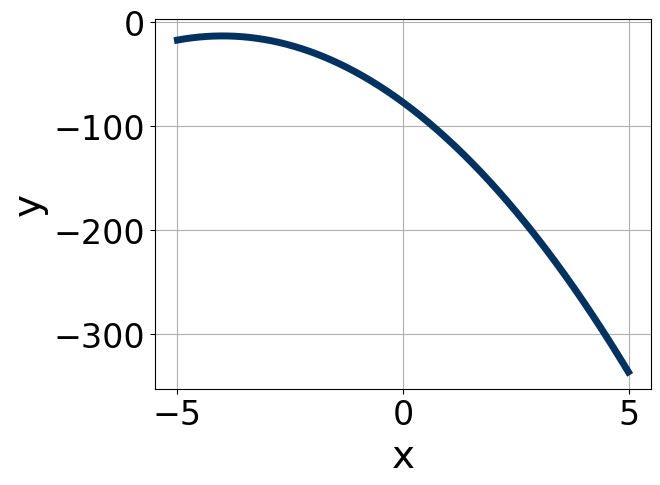
\includegraphics[width = 0.3\textwidth]{../Figures/quadraticEquationToGraphCopyAB.png}\item 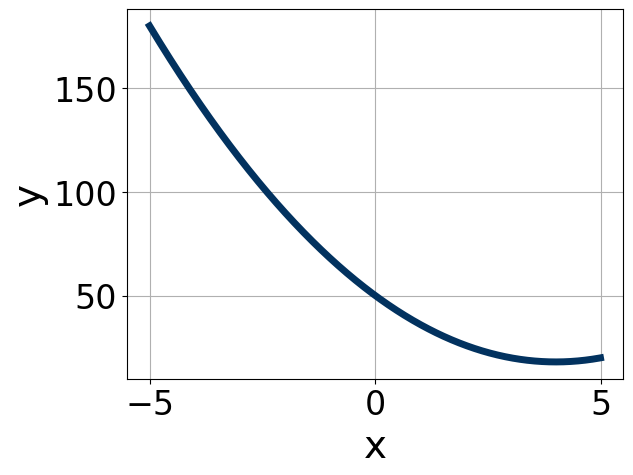
\includegraphics[width = 0.3\textwidth]{../Figures/quadraticEquationToGraphCopyBB.png}\item 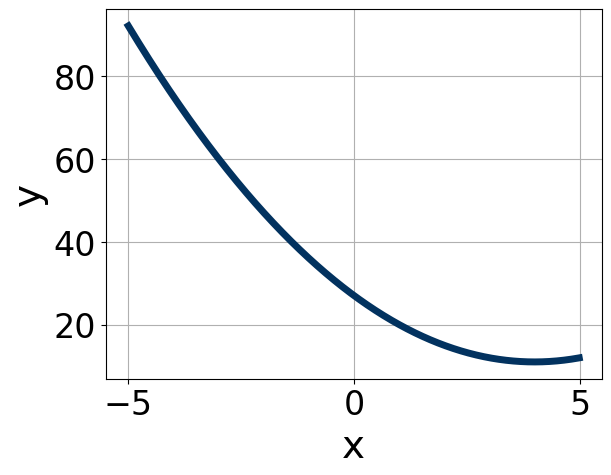
\includegraphics[width = 0.3\textwidth]{../Figures/quadraticEquationToGraphCopyCB.png}\item 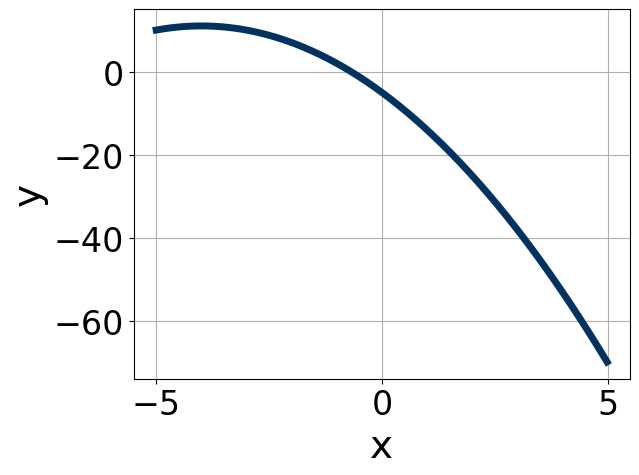
\includegraphics[width = 0.3\textwidth]{../Figures/quadraticEquationToGraphCopyDB.png}\end{multicols}\item None of the above.
\end{enumerate} }
\litem{
Solve the quadratic equation below. Then, choose the intervals that the solutions belong to, with $x_1 \leq x_2$ (if they exist).\[ -15x^{2} -11 x + 3 = 0 \]\begin{enumerate}[label=\Alph*.]
\item \( x_1 \in [-3.2, -1.77] \text{ and } x_2 \in [13.03, 14.69] \)
\item \( x_1 \in [-18.06, -17.49] \text{ and } x_2 \in [16.38, 17.64] \)
\item \( x_1 \in [-0.25, 0.19] \text{ and } x_2 \in [0.47, 2.44] \)
\item \( x_1 \in [-1.45, -0.57] \text{ and } x_2 \in [0.14, 0.22] \)
\item \( \text{There are no Real solutions.} \)

\end{enumerate} }
\litem{
Solve the quadratic equation below. Then, choose the intervals that the solutions belong to, with $x_1 \leq x_2$ (if they exist).\[ -18x^{2} -12 x + 3 = 0 \]\begin{enumerate}[label=\Alph*.]
\item \( x_1 \in [-4.06, -2.84] \text{ and } x_2 \in [15.48, 15.53] \)
\item \( x_1 \in [-0.22, -0.12] \text{ and } x_2 \in [0.23, 0.99] \)
\item \( x_1 \in [-19.88, -18.89] \text{ and } x_2 \in [18.28, 18.76] \)
\item \( x_1 \in [-1.52, -0.7] \text{ and } x_2 \in [-0.67, 0.77] \)
\item \( \text{There are no Real solutions.} \)

\end{enumerate} }
\litem{
Write the equation of the graph presented below in the form $f(x)=ax^2+bx+c$, assuming  $a=1$ or $a=-1$. Then, choose the intervals that $a, b,$ and $c$ belong to.
\begin{center}
    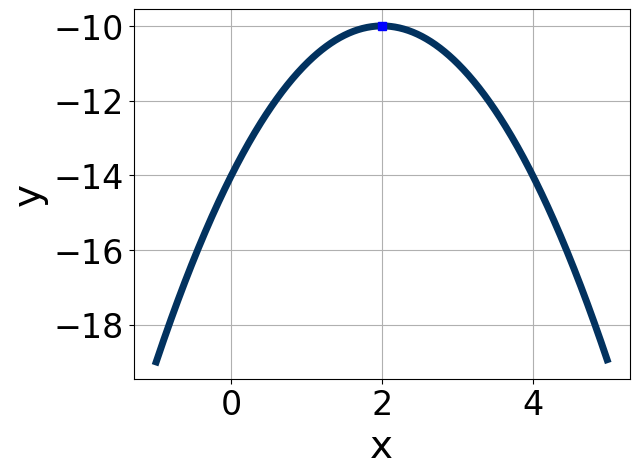
\includegraphics[width=0.5\textwidth]{../Figures/quadraticGraphToEquationB.png}
\end{center}
\begin{enumerate}[label=\Alph*.]
\item \( a \in [0.6, 2.8], \hspace*{5mm} b \in [-7, -3], \text{ and } \hspace*{5mm} c \in [2, 4] \)
\item \( a \in [-2.5, -0.8], \hspace*{5mm} b \in [-7, -3], \text{ and } \hspace*{5mm} c \in [-8, -5] \)
\item \( a \in [-2.5, -0.8], \hspace*{5mm} b \in [2, 5], \text{ and } \hspace*{5mm} c \in [-8, -5] \)
\item \( a \in [0.6, 2.8], \hspace*{5mm} b \in [2, 5], \text{ and } \hspace*{5mm} c \in [2, 4] \)
\item \( a \in [-2.5, -0.8], \hspace*{5mm} b \in [2, 5], \text{ and } \hspace*{5mm} c \in [-2, 1] \)

\end{enumerate} }
\litem{
Factor the quadratic below. Then, choose the intervals that contain the constants in the form $(ax+b)(cx+d); b \leq d.$\[ 24x^{2} +2 x -15 \]\begin{enumerate}[label=\Alph*.]
\item \( a \in [0.4, 1.9], \hspace*{5mm} b \in [-21, -17], \hspace*{5mm} c \in [-1.2, 1.1], \text{ and } \hspace*{5mm} d \in [19, 21] \)
\item \( a \in [7.9, 9.9], \hspace*{5mm} b \in [-3, 2], \hspace*{5mm} c \in [1.2, 3.2], \text{ and } \hspace*{5mm} d \in [1, 7] \)
\item \( a \in [0.4, 1.9], \hspace*{5mm} b \in [-3, 2], \hspace*{5mm} c \in [16.8, 20.9], \text{ and } \hspace*{5mm} d \in [1, 7] \)
\item \( a \in [2.4, 5.1], \hspace*{5mm} b \in [-3, 2], \hspace*{5mm} c \in [3.6, 6.7], \text{ and } \hspace*{5mm} d \in [1, 7] \)
\item \( \text{None of the above.} \)

\end{enumerate} }
\litem{
Write the equation of the graph presented below in the form $f(x)=ax^2+bx+c$, assuming  $a=1$ or $a=-1$. Then, choose the intervals that $a, b,$ and $c$ belong to.
\begin{center}
    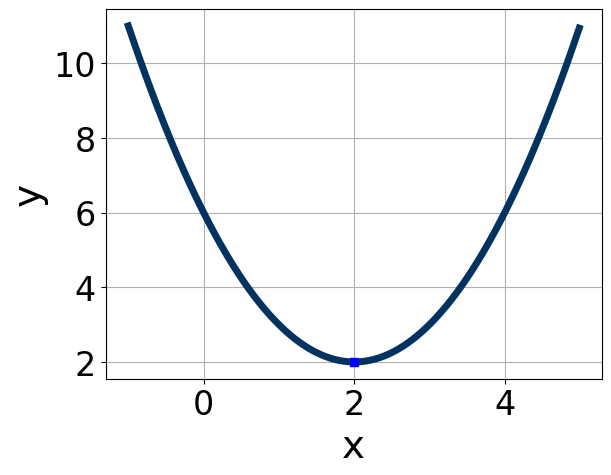
\includegraphics[width=0.5\textwidth]{../Figures/quadraticGraphToEquationCopyB.png}
\end{center}
\begin{enumerate}[label=\Alph*.]
\item \( a \in [0.2, 1.8], \hspace*{5mm} b \in [1, 5], \text{ and } \hspace*{5mm} c \in [-6, -3] \)
\item \( a \in [-1.6, -0.9], \hspace*{5mm} b \in [-8, -2], \text{ and } \hspace*{5mm} c \in [-14, -11] \)
\item \( a \in [-1.6, -0.9], \hspace*{5mm} b \in [1, 5], \text{ and } \hspace*{5mm} c \in [2, 6] \)
\item \( a \in [0.2, 1.8], \hspace*{5mm} b \in [-8, -2], \text{ and } \hspace*{5mm} c \in [-6, -3] \)
\item \( a \in [-1.6, -0.9], \hspace*{5mm} b \in [1, 5], \text{ and } \hspace*{5mm} c \in [-14, -11] \)

\end{enumerate} }
\litem{
Graph the equation below.\[ f(x) = -(x-1)^2 - 12 \]\begin{enumerate}[label=\Alph*.]
\begin{multicols}{2}\item 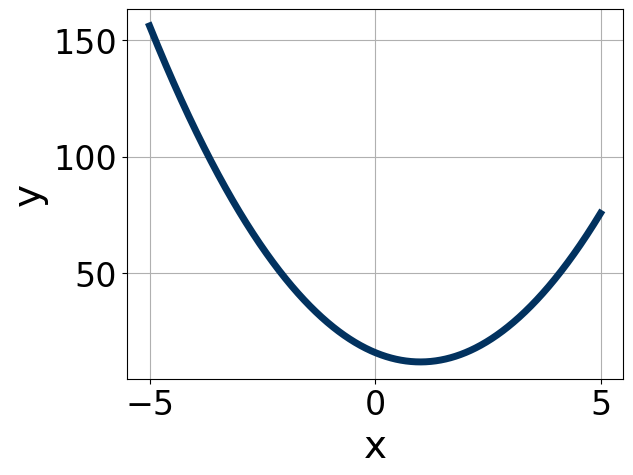
\includegraphics[width = 0.3\textwidth]{../Figures/quadraticEquationToGraphAB.png}\item 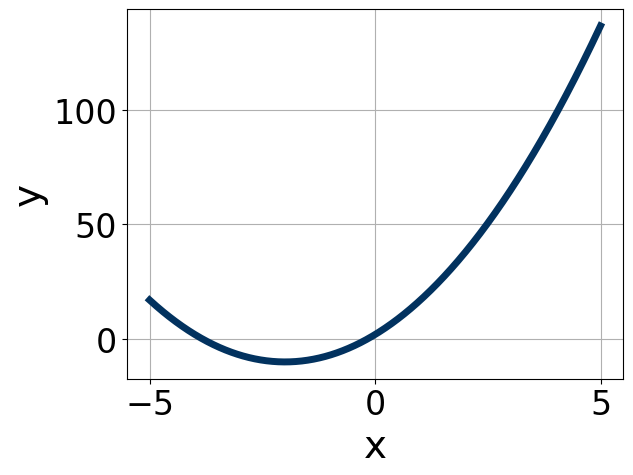
\includegraphics[width = 0.3\textwidth]{../Figures/quadraticEquationToGraphBB.png}\item 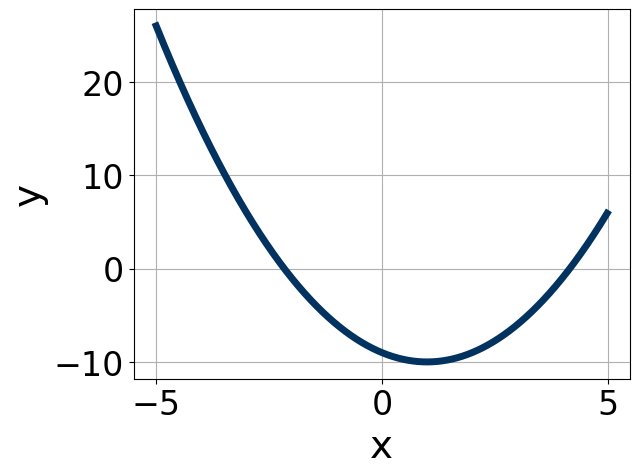
\includegraphics[width = 0.3\textwidth]{../Figures/quadraticEquationToGraphCB.png}\item 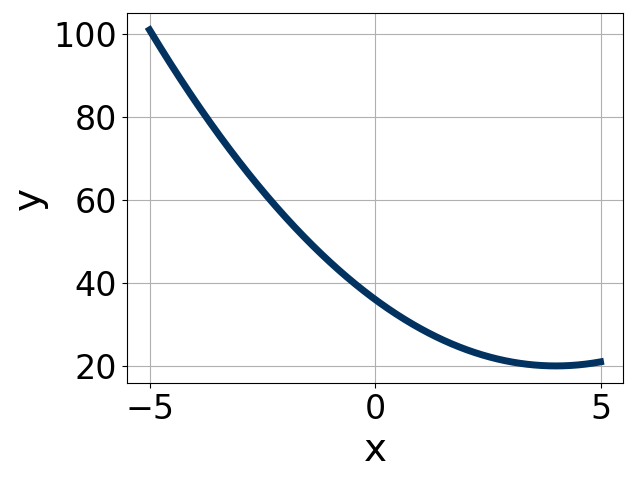
\includegraphics[width = 0.3\textwidth]{../Figures/quadraticEquationToGraphDB.png}\end{multicols}\item None of the above.
\end{enumerate} }
\end{enumerate}

\end{document}